\documentclass[12pt, a4paper, oneside]{ctexart}
\usepackage{fancyhdr}
\usepackage{amsmath, amsthm, amssymb, bm, graphicx, hyperref, mathrsfs, graphicx, float, subfigure, caption, makecell, longtable,framed,booktabs}
\usepackage[dvipsnames]{xcolor}
\usepackage{listings}
\renewcommand{\lstlistingname}{Code}
\lstset{
    language=C++, % 设置语言
 basicstyle=\ttfamily, % 设置字体族
 breaklines=true, % 自动换行
 keywordstyle=\bfseries\color{NavyBlue}, % 设置关键字为粗体,颜色为 NavyBlue
 morekeywords={}, % 设置更多的关键字,用逗号分隔
 emph={self,input,output,wire,reg,posedge,negedge}, % 指定强调词,如果有多个,用逗号隔开
    emphstyle=\bfseries\color{Rhodamine}, % 强调词样式设置
    commentstyle=\itshape\color{black!50!white}, % 设置注释样式,斜体,浅灰色
    stringstyle=\bfseries\color{PineGreen!90!black}, % 设置字符串样式
    columns=flexible,
    numbers=left, % 显示行号在左边
    numbersep=2em, % 设置行号的具体位置
    numberstyle=\footnotesize, % 缩小行号
    frame=single, % 边框
    framesep=1em % 设置代码与边框的距离
}
\renewcommand\thesubsection{\zhnum{subsection}、}
\renewcommand\thesubsubsection{\arabic{subsubsection}.}
\renewcommand\theparagraph{(\arabic{paragraph})}
\renewcommand\thesection{}
\usepackage[left=1in, right=1in, top=1in, bottom=1in]{geometry}

\pagestyle{fancy}
\fancyhf{}
\renewcommand{\headrulewidth}{0pt}
\fancyfoot[C]{\thepage}

\title{\textbf{ARM开放项目——多功能可调数字时钟}}
\author{张浩宇 522031910129}
\date{}

\begin{document}
    \maketitle
    \subsection{项目简介}
    本项目预期实现一个多功能可调数字时钟,具有以下基本功能:
    \begin{enumerate}
        \item 时钟功能:在数码管显示时间,并可以调整时间;
        \item 闹钟功能:可以设定闹钟,到时间后会响铃;
        \item 秒表功能:可以计时,并在数码管显示计时时间。
    \end{enumerate}
    \subsection{功能设计}
    该时钟具有四种模式:普通模式、时间设置模式、闹钟设置模式和秒表模式。
    按键\verb|USR_SW1|和\verb|USR_SW2|为交互按键,按下按键以进行各种操作,且按下时伴有蜂鸣器音,
    \verb|LED_M0|~\verb|LED_M3|为状态指示灯。
    \subsubsection{普通模式}
    开机后处于普通模式,\verb|LED_M0|亮起指示当前为普通模式,
    此时数码管以“HH-MM-SS”形式显示当前时间。
    \subsubsection{时间设置模式}
    在普通模式下短按\verb|USR_SW1|进入时间设置模式,
    \verb|LED_M1|亮起指示当前为时间设置模式,
    此时可以调节时间。在时间设置模式下,短按\verb|USR_SW1|切换调节项,当前调节项会闪烁以指示,
    初始为时,按下后切换到分,再按下切换到秒,此时再按将退出,回到普通模式;
    短按\verb|USR_SW2|使当前调节项数值+1。
    \subsubsection{闹钟设置模式}
    在普通模式下短按\verb|USR_SW2|进入闹钟设置模式,\verb|LED_M2|亮起指示当前为闹钟设置模式。
    此时可用与时间设置相同的方式设置闹钟时间,但闹钟仅可以设置时和分,数码管显示当前设置闹钟时间,
    调节项为分时再按\verb|USR_SW1|将退出,回到普通模式,将此时设置的时间作为闹钟时间,且\verb|led1|亮起,
    指示当前闹钟已经设置。

    当时间到达闹钟设置时间时,蜂鸣器将响起,同时LED1闪烁。结束后LED1不再亮起,指示当前闹钟已无闹钟。
    \subsubsection{秒表模式}
    在普通模式下长按\verb|USR_SW1|进入秒表模式,\verb|LED_M3|亮起指示当前为秒表模式,
    此时数码管时间显示为0,再短按\verb|USR_SW1|开始计时,数码管上显示“分-秒-毫秒”。在计时开始时,
    短按\verb|USR_SW1|暂停计时,并通过UART发送当前计时时间,短按\verb|USR_SW2|会发送按下时的计时时间,且计时保持进行;
    当计时暂停时,长按\verb|USR_SW2|将计时清零,长按\verb|USR_SW1|将退出,回到普通模式。
    \subsubsection{UART命令控制}
    除了按键,还可通过UART串口发送命令的方式进行控制,此方式不受当前模式的影响。
    \begin{enumerate}
        \item 发送“SETXX:XX:XX”:直接设置为当前时间;
        \item 发送“INCXX:XX:XX”:在当前时间上增加时间;
        \item 发送“ALARMXX:XX:XX”:直接设置为当前闹钟时间;
        \item 发送“GETTIME”:返回当前时间。
    \end{enumerate}
    \subsection{功能实现}
    \begin{figure}[h]
        \centering
        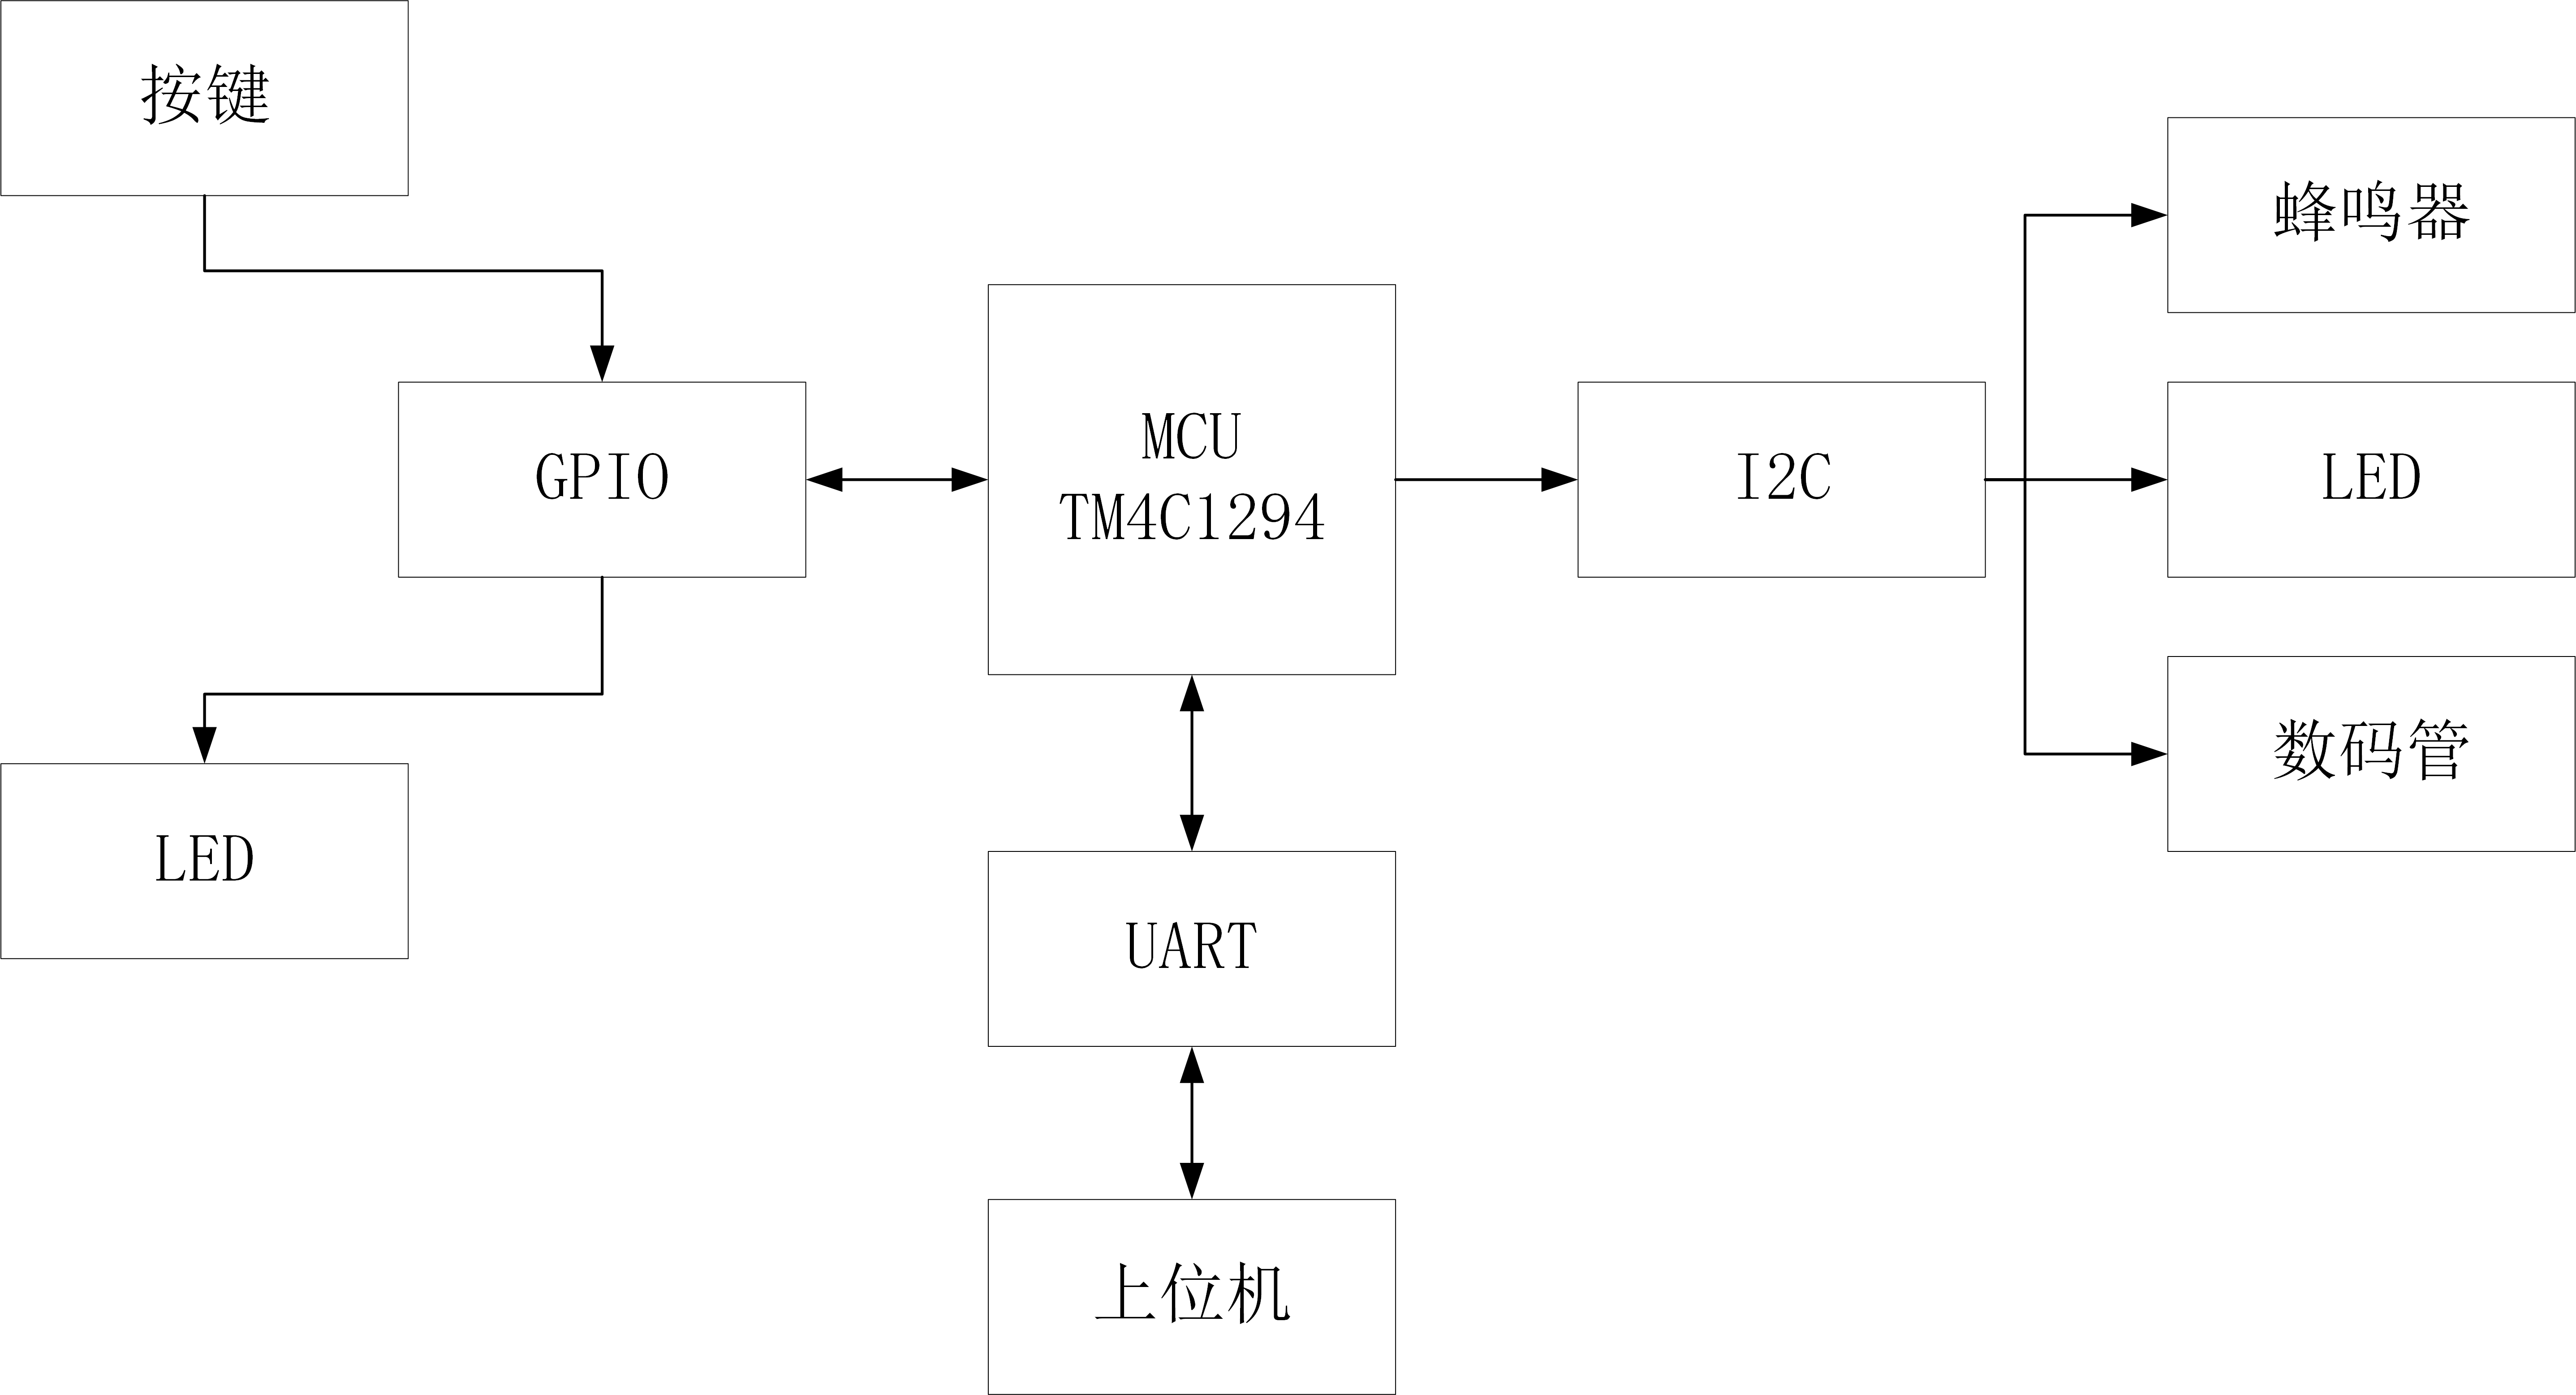
\includegraphics[width=0.8\textwidth]{./img/system.png}
        \caption{系统框图}
        \label{fig:system}
    \end{figure}
    系统框图如图\ref{fig:system}所示。系统由GPIO按键和UART串口通信
    来进行人机交互,通过I2C扩展IO来驱动数码管和蜂鸣器,并通过GPIO和I2C上的
    一系列LED来指示系统状态。



    

    \subsection{结果展示}
     
\end{document}

